\section{Parameterized approach}

\subsection{Introduction}

The Parameterized approach concludes that all plants function the same way on a
certain level and all that is really needed to describe a plant is to set some
parameters for this universal algorithm. A plant would then consist of a set
of parameters. All that is left is to sort out these parameters, find an 
appropriate level and write the algorithm.

\subsubsection{Common tree features}
In order to structure the describing language, common features are sought out.

\paragraph{Levelized architecture}
Plants and especially trees have a strong tendency to possess a level-like
structure. Considering the trunk or perhaps root as the bottomlevel, levels
of branches are applied in a hierarchical order, ending with a toplevel
consisting of leaves. Although it does vary, the number of branchlevels
leading up to a leaf is strikingly constant throughout a grown-up tree. This
probably due to the fact that a leaf with a lesser number of sublevels are
inclined to be shaded from the sun by leaves sprouting from a deeper
branch-hierarchy, since those are likely to be farther out and of greater 
numbers. 

\paragraph{Branchlevel similarity}
Branches belonging to the same level often seem to share a number of
properties, such as growth-angle from motherbranch and spawning statistics. 

\subsubsection{Distinguishing tree features}
As the common features are considered when designing the static parts and syntax of the 
language, the individualizing properties will be reflected upon the dynamic
parameterized parts.

\paragraph{Branchleveling}
Given a certain branchlevel, how often is it inclined to spawn a childbranch
of which sort.

\paragraph{Branchdistributioning}
How much energy does a branch use up on itself and how much does it pass on to
its children.

\paragraph{Branchshape}
Physical shape of the branch.

\paragraph{Treeshape}
The overall impression of the tree's physical shape. Typically columnar, cone,
distributed or blobbed.

\paragraph{Constraints}
Is a childbranch allowed to grow further than the motherbranch, or perhaps no
more than 30\% of the total motherbranch development?

\subsubsection{Meta-language characteristics}
Considering the aforementioned properties of trees, the components of the 
top-level language where decided to be stack-leveled, that is
branch-descriptions are stacked in the order they appear on the tree. A branch 
will spawn all branches which are lower on the stack (the trunk being the top 
element). Stack elements contain an interface which says how that level is
attached to its motherlevel, and a plant node expressing the properties of
instances of the level.

\paragraph{Interface}
The \emph{interface} contains information about \emph{branch distribution}, 
determining the overall shape of that level. \emph{Spawn count}, for instance 
pines may spawn several sprouts at the same time, creating branchrings. \emph{Angle 
distribution}, angle in relation to its mother and the upvector. \emph{Evolution}, 
determines when the level spawns. \emph{Energy modification}, constraints on 
how the level may grow.

\paragraph{Plant Node}
A \emph{plant node} characterizes the \emph{shape} of the level.
\emph{Elasticity}, determining gravitational displacement. Possibly also
\emph{texture} and \emph{size} if the node is a leaf.

\paragraph{}
The seed of a simple tree could be then be thought as a stack of
(interface, node)-tuples:
\\\\
{\bf (trunk interface, trunk node)\\
(branch interface, branch node)\\
(leaf interface, leaf node)}

\subsubsection{Chaotic behaviour of nature}
Regarding nature as a system, it has chaos properties. That is, although in
some sense deterministic, it may require a very large number of variables
with arbitrarily high precision in the equation necessary to calculate 
its behaviour and state. Its
affect on a plant appears to have random properties, yet dominated by major
factors such as temperature and sunlight exposure. This randomness on a
low-level, however suggests that randomness should be employed to work on the
shaping of a tree.

\subsection{Meta language}
\subsubsection{Ambition and structure}
The aim was set to create a language, which on the toplevel would be very
intuitive and easy to use. The branching structure and types would be set with
a set of base-components, which should suffice to create a number of basic
treetypes. Using a set of modifiers and a library of more lowlevel components
the seed can be further modified to a desired behaviour. On the base of each 
seed is an \emph{earth}-component that contains
the root function and other general information. The '<<'-operator simply
binds the branchlevels in a hierarchical order. Conceptual examples
below. 
\\\\
\begin{tabular}{ll}
  &StdEarth\\
  <<&(trunk-interface, pine-trunk)\\
  <<&(ring-interface, straight-branch)\\
  <<&(horizontal-interface, straight-branch)\\ 
\end{tabular}
\\\\
\emph{Basic model of a pine tree}\\

\begin{tabular}{ll}
  &StdEarth\\
  <<&(trunk-interface, modThickness 5.0 \$ pine-trunk)\\
  <<&(modDistribution triangleFunc \$ ring-interface, straight-branch)\\
  <<&(horizontal-interface, straight-branch)\\ 
\end{tabular}
\\\\
\emph{Modifying the basic model of a pine tree. Setting thickness property to
5.0 and the general shape of the tree to a triangular one}

\subsubsection{Language Levels}
\begin{enumerate}
\item
Toplevel language "MetaPlant", a set of combiners and basic factors.
\item
Modifiers with parameter library. Extends the toplevel language.
\item
Lowlevel library components. Buildingblocks for the parameter library.
\item
Host language datatype constructors. Haskell constructs derived from the
toplevel language.
\end{enumerate}

\subsubsection{Randomness}
As suggested above each BranchState contains a random seed, accessible by the
shaper functions which can ensure that branches are given unique
representations.

\subsubsection{Libraries}
There are a set of standard interfaces and standard branches, for typical tree
paradigms, such as leaf and pine trees. These sometimes take a few arguments 
that set the starting growth angle interval, the size and texture of a leaf or
the wigglyness of a branch. These standard components are then modified by
adding replacing properties with modifiers. Typically, one would like to change
the shape of the tree with a new distribution function. The modifier may take
completely new function, but in most cases a constructor-function is used, which only
take some essential parameters and hides away the ugliness of the process. In
the distributor case the essential parameters would be constituted of a function
that takes the development of the branch at a certain place and says what mass concentration should
be at that level. Sometimes the normalized position (position in relation to
entire length) is more suitable, for instance when a tree is supposed to look
the same its entire life (a spruce maybe), where as a function such as (\\rel\_pos
-> 1.0 - rel\_pos) would be deployed (0.0 being near root and 1.0 near the top).

\subsubsection{Limitations}
Although the seed may be extensively configured the heart of the behaviour is
still in the simulation-module which may not be modified. Some things regarding
the life of the plant may thus not be changed. For example, when power is low
the plant will inevitably attempt to sustain the leaves closest to the root and
not the other way around. A branch may not switch plant id (identifying the
internal type of branch). If a branch falls off the tree, it will never grow out
again.

\subsection{Simulation}
The simulation algorithm takes the current state of the tree, an environment
and the time to run. The root-function converts the environment to power that
is sent throughout the plant according to the interfaces of the branches.
\subsubsection{Overview}
Beginning at the trunk the following steps are taken:
\paragraph{Vitalize leaves} 
It is feasible to assume that the trees first priority is to feed its leaf,
since they are essential for the photosynthesis that generates the carbon
substances needful for further development of the plant.
\paragraph{Feed the child branches} 
Power is disposed according to the distribution
function, that determines the overall shape of the plant. Each child is then
simulated recursively with its granted power.
\paragraph{Simulate forces of nature} 
The forces and corrosive powers of nature are taking affect on the current
level.
\paragraph{Evolve this branch}
Use granted power to develop branch and add new
children.

\subsubsection{Preparations}
The environment, including resources, temperature and other peripheral factors
are passed to the simulation step along with the time to run. Each plant then
have a root function, which converts the given environment to the fictive unit
growth-power. Since the power remains static during the simulation step; it is
important that a higher function creates environment-wise fine-tuned intervals
for a believable evolution. Together with the root-function-evaluated power,
there may be unused, accumulated power from previous steps which are added to
the power-pool. To generalize the concept of resources to a single powerunit
might seem limiting, but has proven quite satisfactory and simplifies the
underlying methods. There are even some possibilities to at the bottomlevel
take heed to the surrounding environment, when using a development modification
function, that at the lowest level can modify the development of a branch.\\\\
In the case that it is the first-time simulation-step for the given plant, a
special genesis-path is taken, which setup the infant trunk-level branch with
seed according parameters, the most important being the event list.
\\\\
Further more, before the actual powerdistribution takes place, some flags are
set and the simulation state initialized.

\subsubsection{Power distribution - discussion}
Each seed has at each level a function that says how much of the total
mass on a level should be concentrated to each branch. That is, for each of
the attached branch, a mcn (mass-concentration-number) is generated from the
seeds distribution function on that level. For a pine tree it
would typically somewhat triangular, $f = 1 - x$, where x is the relative
position on the motherbranch $\frac{position}{mothers development}$ and for a tree 
with columnar shape near
constant $f = 1.0$. A strangely shaped tree may wish to use absolute coordinates
to shape sharp and steady contours.
\\\\
Ideally, the power, $p_{incoming}$, will attempt to fulfill:
$p_{incoming}=\frac{d}{dt}(w_{reference} - w_{current})$, with $w_{reference}$
being the mass according to the distribution function and the $w_{current}$
the actual current mass distribution, mass by definition equaled to energy. 
It is however, and for several reasons, impossible to use this formula, the 
functions not being derivable for one thing. Hence, approximations must be
explored.
\\\\
Alot of approaches was attempted in order to find a strategy with the sought-
for-properties. The necessary features includes maintaining the shape defined
by the seed, promoting self-survival and perhaps most difficult - not loosing
any power throughout the distribution flow. 
\\\\
The naive way to distribute would be to simply calculate the
mcn for each subbranch at the current level,
normalize them and multiply with the available power, assuming that all power
will be transformed into mass, in one way or another. There may however be
branches that cannot consume the power given to them, due to restrictions of
strength (or other), then something must be done with the excessive power. 
One strategy is to store the excessive power returned by the children at the 
motherbranch and then simply add it to the incoming power next round. If the 
tree is growing and the distribution depends mostly on relative position (which 
then changes rapidly), this scheme is quite useful, but proves to end up 
accumulating vast 
amounts of power at certain branches is most cases. Countermeasures against
this sort of powertraps may begin with regarding how much power a certain
branch fed the last cycle and adapting the current flow to match if it was
minor. This power limit must however be updated at some point,
since it may very well be that the branch will be able to accept more power
in future times. Thus the powertrap persists. One solution would be to raise
the powerlimit gradually and thereby decreasing the unwanted power buildup.
This, although working with reasonable result introduces uninvited latency to
the system, breaking the distribution model.
\\\\
Another issue one must take into account when contemplating the distribution
is the fact that the prerequisites that determined the current distribution 
change after the new power has been deployed. That is - the calculated
distribution is really only valid for the first infinitesimal bit of power. As
soon it is consumed it changes the mass-distribution and thereby the desired
power-distribution.
\\\\
The perhaps most obvious solution would be simply to chop the simulation
timeframe into very small portions, which well approximates the infinitesimal
criteria. This however is very time consuming, since running the simulation is
a time-expensive operation no matter the distribution issue solved. In stead,
the timeframe partitioning is left to a higher level.
\\\\
The difficulties in not loosing any power has made itself heard on
implementation level.

\subsubsection{Power distribution - working strategy}
Testing of several models with regards to above arguments lead up to a method
working in multiple stages. It is assumed that the timeframe of each
simulation step is relatively short.
\paragraph{Feed to equilibrium}
In the first step, an attempt is made to bring justice to the branches. The
power difference $w_{reference} - w_{current}$ is computed (values clamped to
$[0..\infty]$, we don not want backwards growth). Probing each of the
potential branches (those given a non zero, positive distribution) only those
branches ready to accept more power are selected and then the power
converted to mass is used to neutralize the power difference in those
branches. The probing mechanism is provided by sending some small amount of
power to the simulation functions of the branches, detecting whether it
is bounced back or not. The power sent to the branches may partly bounce back,
should the branched be saturated. That power will be stored and used in the
next step.
\paragraph{Feed the hungry}
Given that any power remains when the assumed equilibrium is reached, the
branches are once again probed, and the remaining power is sent throughout the
hungry branches in accordance with the distribution.
\paragraph{Feed thy self}
The remaining power (including the one rejected in the second step) is used to
evolve the current branch. The power rejected on the current level is passed
back to the superlevel, and if the current level happen to be the baselevel
the power is accumulated and added to the incoming power next time around.
Therefor it is important not to use to great steps or December may become
sunny as June.

\subsubsection{Regulators}
Intuitively it might seem tempting to view the tree as a dynamic system and
deploy regulators to control it. Simplified, the system would then preferably be
represented as the following illustration.

\begin{figure}[htb]
        \centering
        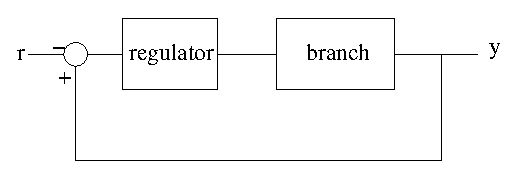
\includegraphics[height=2cm,width=6cm, angle=0]{images/regulsimple}
        \label{fig:db:graph1}
\end{figure}

Here, a PI-regulator would seem fitting to steer the power going into the
current branch.

However, because of the modifier preceeding the branch, the behaviour of the branch 
is not as depending on the insignal as would have to for this to work.

The implemented solution would by similar methods be illustrated as follows.
 
\begin{figure}[htb]
        \centering
        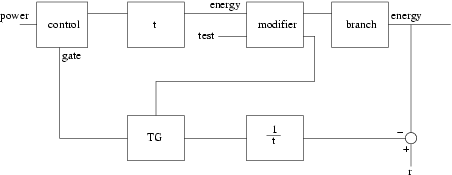
\includegraphics[height=5cm,width=12cm, angle=0]{images/regulsys}
        \label{fig:db:graph2}
\end{figure}

Note how the probe signal ('test' in the figure) opens the feedback loop if the
probe is successful. This is indeed more or less a plain P-regulator, making use
of several ingoing signals to the system.
 
\subsubsection{Evolving the current branch}
Each branch has an event list which includes events with attached development
stamps, stating at which level of development the events will activate. The
events are different sub-branchings, where the branch will spawn off new
branchlings. Thus, in order to evolve a certain branch, the following steps
are taken.
\\\\
\emph{Find development of next event}, by parsing the event list. If that
development is not reached within the given timeframe, then simply grow, else
\emph{grow to the development of next event}, subtract the time used from the
timeframe and start over seeking the next event. When the algorithm is
restarted, only the newborn branches are taken into account. The leaves of the
branch is naturally only fed during the first round. 
\\\\
Growing is done by
converting the integrating the power over time and then adding the resulting
mass/development/energy to the current development. Before it is added, the
branch has a chance to use its \emph{development modification function} to
limit or boost the development being added. The typical use being
not to allow a branch to grow longer than its mother has since the
branched was spawned off. It could also be used to encourage certain shapes.

                       
\subsubsection{Creating a new branch}
To spawn a new branch \emph{b} from an event at branch \emph{a}, the seed is inquired of possible
sublevels and at which time they will branch from \emph{b}. These events are
stored in \emph{b}'s eventlist. Other properties such as growth angle, growth
shape are computed and stored. At \emph{a}, the next \emph{b} event is stored.
\subsubsection{Leaves}
Leaves are treated separate from branches, since they do not require the same
care as do the branches. When a leaf has been born, it prospers until the
power is reduced beyond a certain level beyond which it starts to fade away.
When the leaf has faded completely it will fall off the tree. A branch with no
leaves on it will also subsequently fall off the tree. As spring of power
comes, a new leaf will appear where the old one was situated, should the tree
not have grown to thick or otherwise not allow it.

\subsubsection{Approximating the sun}
\paragraph{Effect of the sun}
The leaves not hit by the sun dies. Branches with no leaves dies. 
\paragraph{Emulating the sun}
Find branches that are unlikely to be hit by sun and kill them. Such branches
are recognized by a neighbouring branch which grows slightly above and is 
significantly more developed, since the neighbouring branch is likely 
to shade the other
from the sun due to its greater leaf-area. Leaves in the vicinity of any
branch on the same level dies.
\paragraph{Visual effect}
Thin branches seize to grow close to thick ones.
\subsubsection{Large scale simulation}
It is important to save as much computational power as possible, since the
business of simulation is an expensive one, both on the account of cpu and
memory usage. When it is needful to simulate a larger quantity of trees it is
essential that they share as much simulation structure as possible.
\paragraph{Reuse of simulated structures}
\begin{figure}[htb]
        \centering
        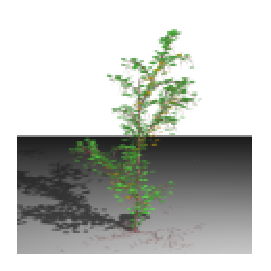
\includegraphics[height=4cm,width=3.5cm, angle=0]{images/clone0}
        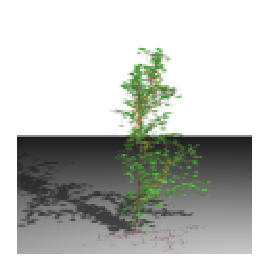
\includegraphics[height=4cm,width=3.5cm, angle=0]{images/clone1}
        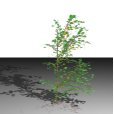
\includegraphics[height=4cm,width=3.5cm, angle=0]{images/clone2}
        \caption{Different clones originating from the same mother}
        \label{fig:clones}
\end{figure}
Assuming that a region have similar properties, it is sufficient to simulate
only one tree, making state snapshots of it at different stages of
development. Consider these trees as a mother set which is used to spawn
clones, by simply changing the random seeds of the branches. To make further
adjustments, parameters as position can be tilted to make the trees
personalized.


\subsubsection{Underlying language specific conceptual issues}
To optimize performance it is needful to utilize destructively mutable arrays
in which to store the branch states. There are several approaches to make this
happen.
\paragraph{ST Monad}
Working in the State-Transformer monad allows for use of the STArray. The STArray 
may however not be exported from the ST monad (to an unstrict environment).
Thus, all array-action must take place within the ST monad, exporting only the
result in a safe form. If the simulation takes place within the ST Monad, no
communication can be done from the outside to the simulation engine. The
resulting simulation is trapped inside ST and exports geometric data in an
infinite list. From the outside the list is pulled and desired models are sent
down the graphics step. Since ST is strict, all geometric data is computed,
not only the one that is used. This is highly undesirable.
\\\\
It is possible to freeze an STArray and thereby converting it to an ordinary
non-strict immutable haskell array. That may in its turn be thawed to an
STArray again within the ST monad, allowing for further use. This can be done
without making copies, using the 'unsafe' operations. It was therefore decided
to remain outside ST everywhere except where it is absolutely necessary, that
is in the inner simulation loop.

\subsection{Visualization}
\subsubsection{Intermediate representation}
In order to visualize a simulation, the simulation representation is first
converted into an intermediate construction, that holds the key properties of
the geometric representation. The intermediate representation may then be
exported to specific standards, such as an OpenGL render section or a collection
of raytracable objects for use with povray or such.

\subsubsection{Processing the Simulated representation}
The simulation representation is constituted of a tree-structure, corresponding
to the actual tree. Therefor, conversion starts at the root, recursively
climbing the branches while updating position and direction of the current
branch. Each branch is represented with a set of cones, whose element count
determines the geometric resolution of the branch. 

\subsubsection{Branch properties}
The thickness of a branch has been decided by the simulation stage, but the
geometry builder makes decisions about how the branch will thin out towards its
end.

\subsubsection{Geometrical resolution}
Obviously, the desired
resolution will vary greatly, depending on closest distance to camera, occluding
geometry and most important - the gradient, or the changing of direction along 
the branch. The constructor will thus increase geometrical resolution when the 
shape is irregular and decrease when the shape tends to be uniform. Leaves are
represented with a simple polygonal surface, with a texture reflecting the
prosperity of the leaf (dying leave are typically low on chlorophyll and thus
yellow or brown in contrast to healthy green).

